\documentclass[tikz,border=2pt,11pt]{standalone}
\usetikzlibrary{arrows.meta}
\usetikzlibrary{positioning}
\usetikzlibrary{calc}
\usepackage{amsmath}
\usepackage{amssymb}
\usepackage{xcolor}
\usepackage{tikz}
\DeclareMathOperator{\Ric}{Ric}
\DeclareMathOperator{\Hess}{Hess}
\DeclareMathOperator{\tr}{tr}
\DeclareMathOperator{\sym}{sym}
\DeclareMathOperator{\supp}{supp}
\DeclareMathOperator{\divg}{div}
\DeclareMathOperator{\id}{id}
\DeclareMathOperator{\rank}{rank}
\DeclareMathOperator{\Lip}{Lip}
\DeclareMathOperator{\Vol}{Vol}
\DeclareMathOperator{\Area}{Area}
\DeclareMathOperator{\dist}{dist}
\DeclareMathOperator{\sgn}{sgn}
\newcommand{\R}{\mathbb R}
\begin{document}
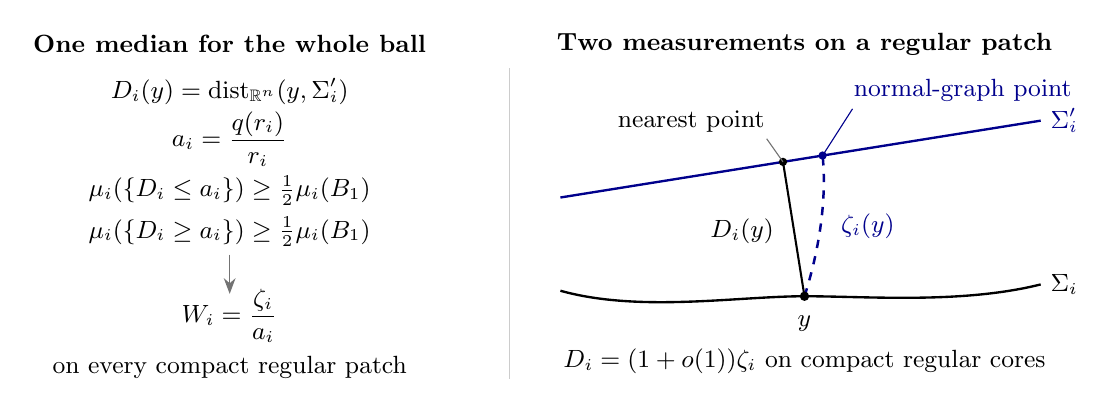
\begin{tikzpicture}[x=1cm,y=1cm,font=\small,
  every node/.style={inner sep=2pt},
  support/.style={line width=.85pt},
  measure/.style={line width=.75pt},
  graphheight/.style={line width=.9pt,dashed,blue!55!black}]
  \node[font=\small\bfseries] at (3.35,4.15)
    {One median for the whole ball};
  \node[font=\small\bfseries] at (10.65,4.15)
    {Two measurements on a regular patch};

  \node[align=center] at (3.35,3.55)
    {$D_i(y)=\dist_{\mathbb R^n}(y,\Sigma'_i)$};
  \node[align=center] at (3.35,2.95)
    {$\displaystyle a_i=\frac{q(r_i)}{r_i}$};
  \node[align=center] at (3.35,2.03)
    {$\mu_i(\{D_i\le a_i\})\ge\tfrac12\mu_i(B_1)$\\[4pt]
     $\mu_i(\{D_i\ge a_i\})\ge\tfrac12\mu_i(B_1)$};
  \draw[-{Stealth[length=2mm]},black!55] (3.35,1.48) -- (3.35,.98);
  \node[align=center] at (3.35,.47)
    {$\displaystyle W_i=\frac{\zeta_i}{a_i}$\\[4pt]
     on every compact regular patch};

  \draw[black!20] (6.9,-.1) -- (6.9,3.85);

  \draw[support] (7.55,1.02)
    .. controls (8.55,.74) and (9.8,.95) .. (10.65,.95)
    .. controls (11.45,.95) and (12.65,.85) .. (13.65,1.1);
  \node[anchor=west] at (13.7,1.1) {$\Sigma_i$};
  \draw[support,blue!55!black] (7.55,2.204) -- (13.65,3.18);
  \node[anchor=west,blue!55!black] at (13.7,3.18) {$\Sigma'_i$};

  \coordinate (y) at (10.65,.95);
  \coordinate (P) at (10.37699,2.65632);
  \coordinate (X) at (10.88,2.7368);
  \draw[measure] (y) -- (P)
    node[pos=.48,left=5pt] {$D_i(y)$};
  \draw[graphheight] (y)
    .. controls (10.82,1.48) and (10.94,2.14) .. (X)
    node[pos=.51,right=5pt] {$\zeta_i(y)$};
  \fill (y) circle (1.7pt);
  \node[below=5pt] at (y) {$y$};
  \fill (P) circle (1.5pt);
  \fill[blue!55!black] (X) circle (1.5pt);
  \node[anchor=south east] at (10.22,2.96) {nearest point};
  \draw[black!55,line width=.4pt] (10.17,2.95) -- (P);
  \node[anchor=south west,blue!55!black] at (11.2,3.35)
    {normal-graph point};
  \draw[blue!55!black,line width=.4pt] (11.26,3.33) -- (X);
  \node[align=center] at (10.65,.12)
    {$D_i=(1+o(1))\zeta_i$ on compact regular cores};
\end{tikzpicture}
\end{document}
